\chapter{First Step with the PortentaH7}

\section{Introduction}
In this chapter we will be looking at how to connect the Arduino Portenta H7 with a PC/laptop in order to use the board. Then, we will be going through the first steps of installing the relevant packages to use the Arduino Portenta H7 board and then we will be implementing a basic example sketch from the Arduino IDE. \cite{portentaSetup:2024}

\section{Configuration}
\begin{figure}
	\begin{center}
		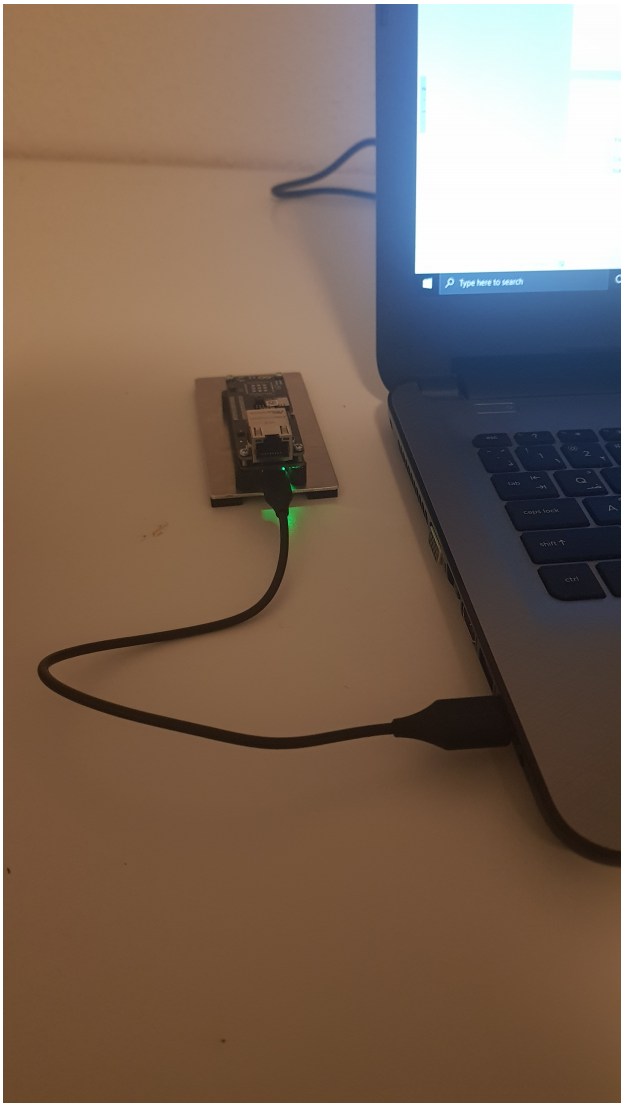
\includegraphics[width=0.3\linewidth]{Images/ArduinoIDE/ArduinoPortentaH7Connectedtoalaptop.png}
		\caption{Arduino Portenta H7 Connected to a laptop}
		\label{ConnetedtoLaptop}
	\end{center}
\end{figure}
\begin{itemize}
	\item Connect the Arduino Portenta H7 board to the computer via USB Type-C cable.
	\item  Press the reset button twice on the board and the LED on the board starts blinking green as shown in the figure \ref{ConnetedtoLaptop} indicating that it is ready.
	\item Next, open the Arduino IDE and navigate to the Boards Manager by selecting \SHELL{Tools > Board > Boards Manager}. In the Boards Manager, search for "Portenta," select \SHELL{Arduino Mbed OS Portenta Boards}, and click "Install". Fig \ref{Installation Arduino Mbed OS Portenta Board} 
\end{itemize} 
	
	\begin{figure}
		\begin{center}
			
			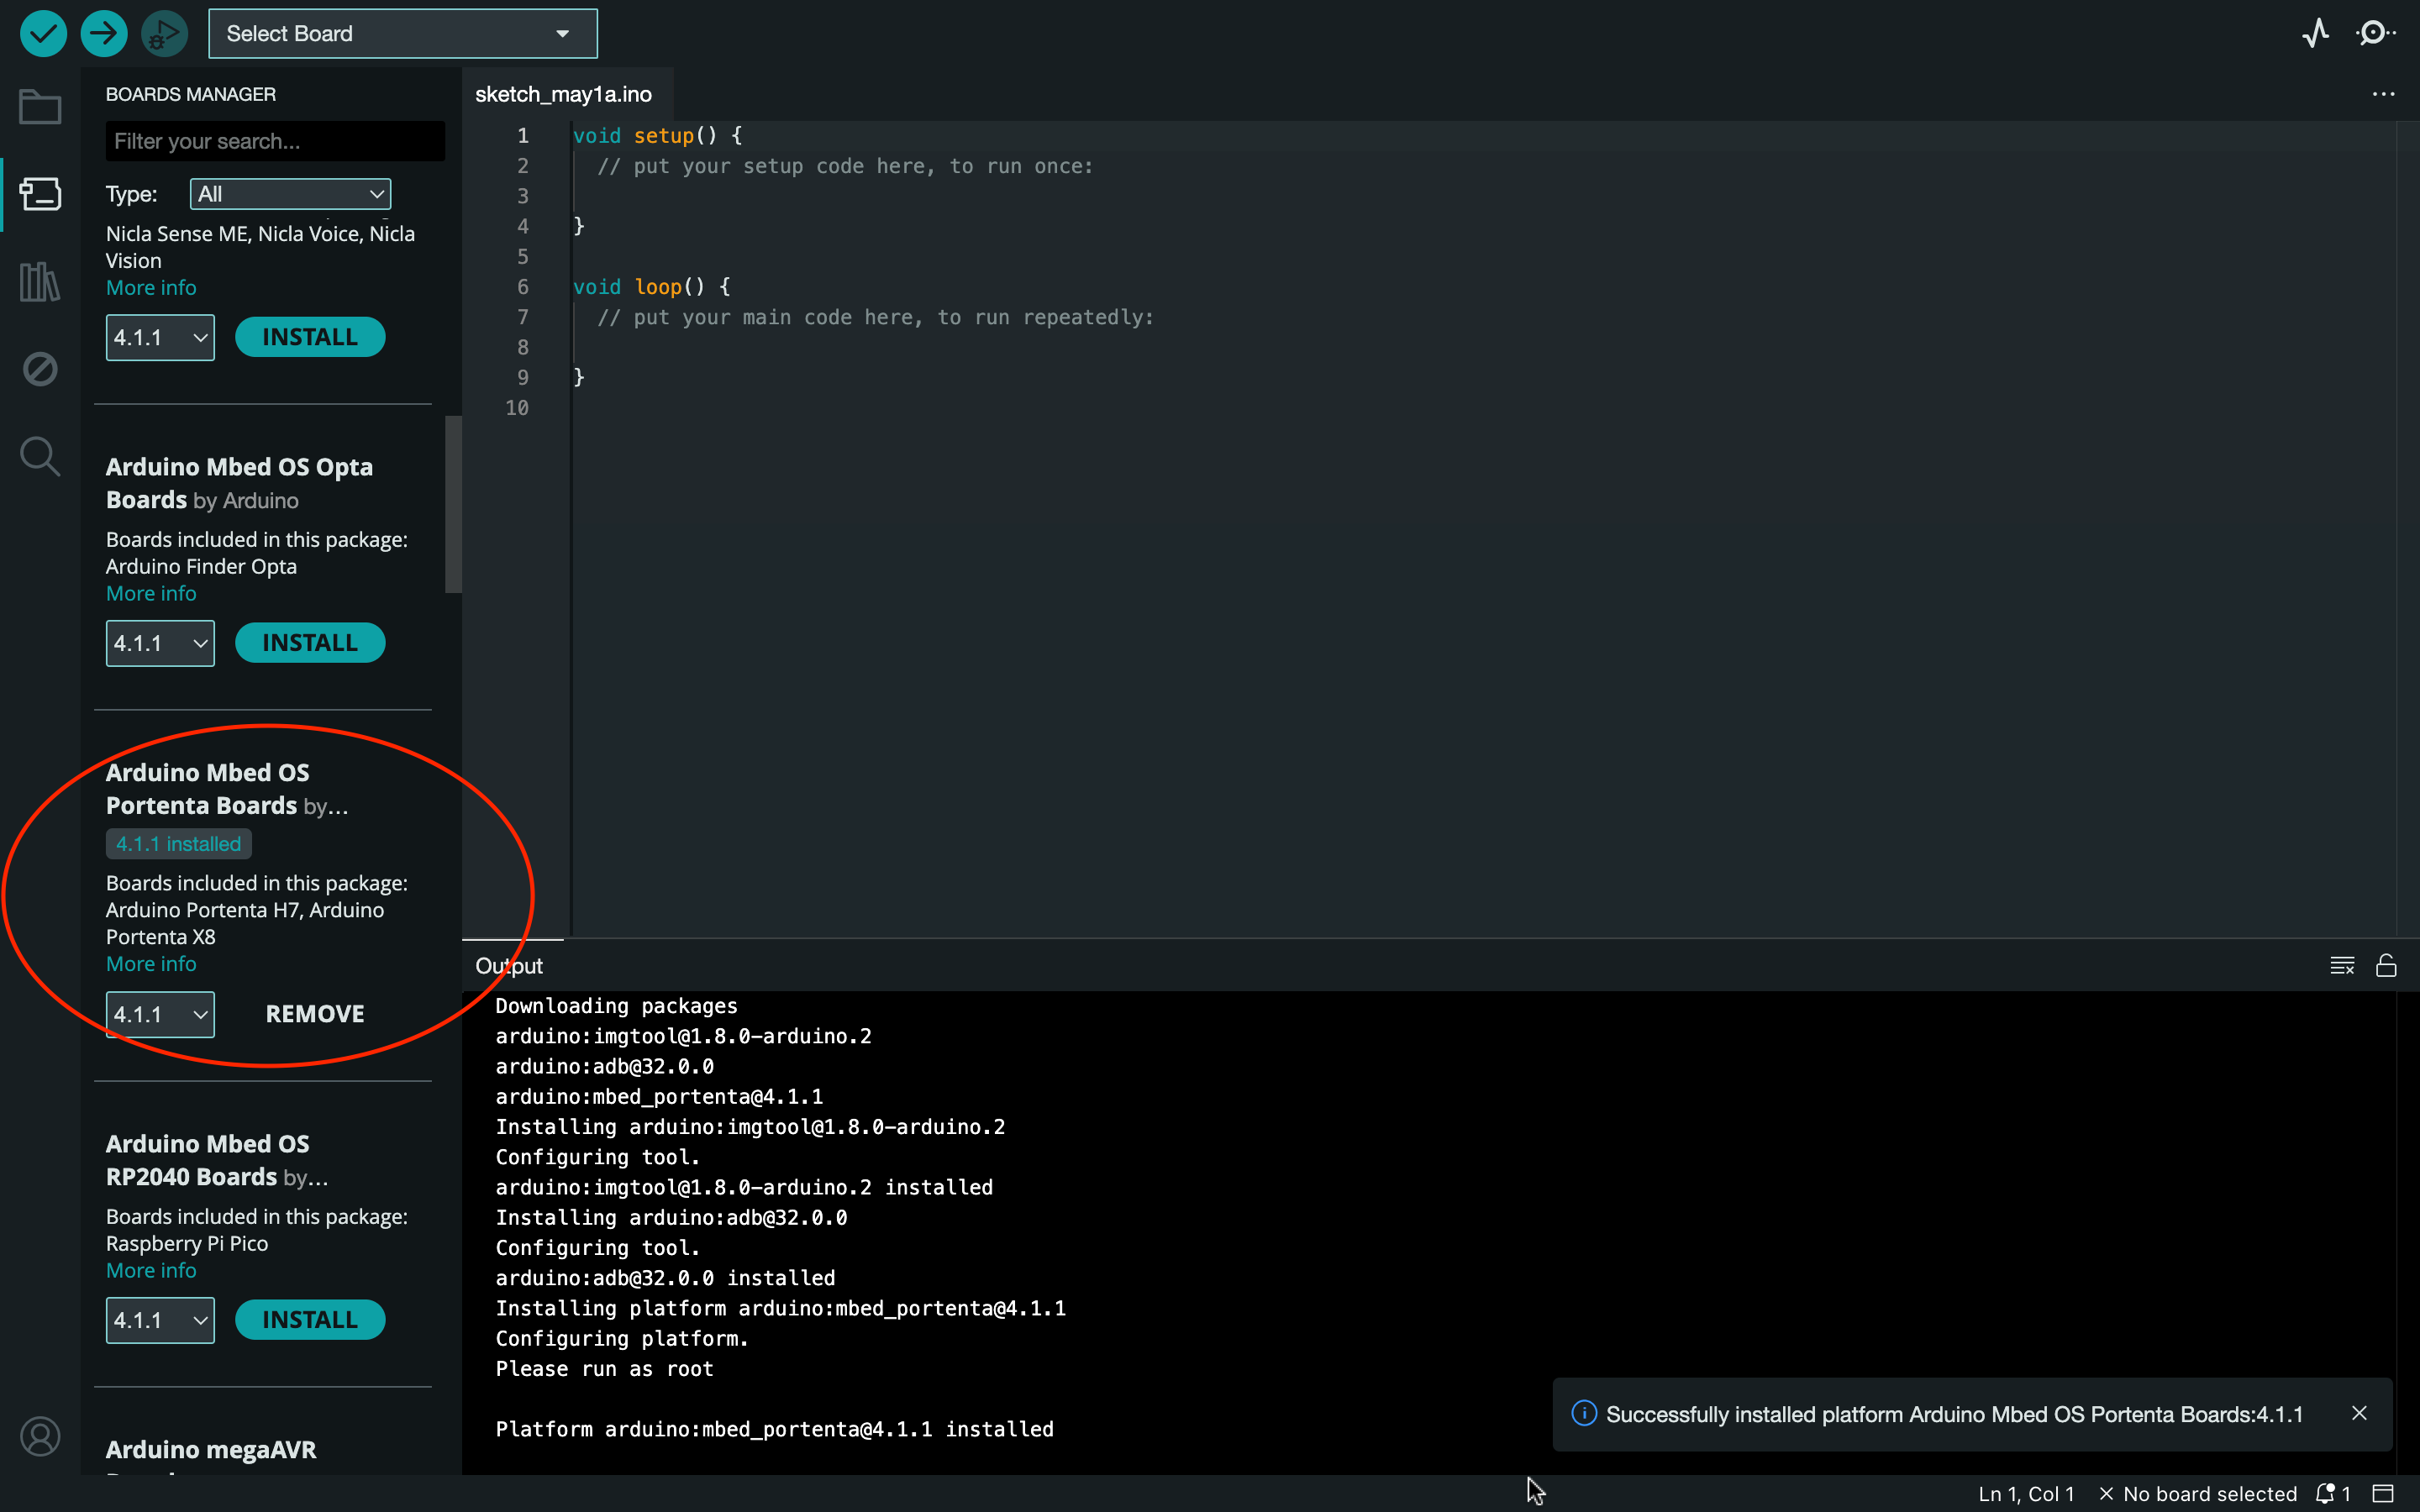
\includegraphics[width=0.7\linewidth]{images/ArduinoIDE/ArduinoMbedOSPortentaBoardsInstallation.png}
			\captionof{figure}{Installation Arduino Mbed OS Portenta Board}
			\label{Installation Arduino Mbed OS Portenta Board}
		\end{center}
	\end{figure}

\begin{comment}
	First we need to install the packages in order to use the Arduino Portenta board. To do this search for Portenta in the boards and select Arduino Mbed OS Portenta Boards and click install as shown in figure \ref{ArduinoPackage} After the installation is done, we can start writing sketches in the IDE.
	
	
	\begin{figure}
		\begin{center}
			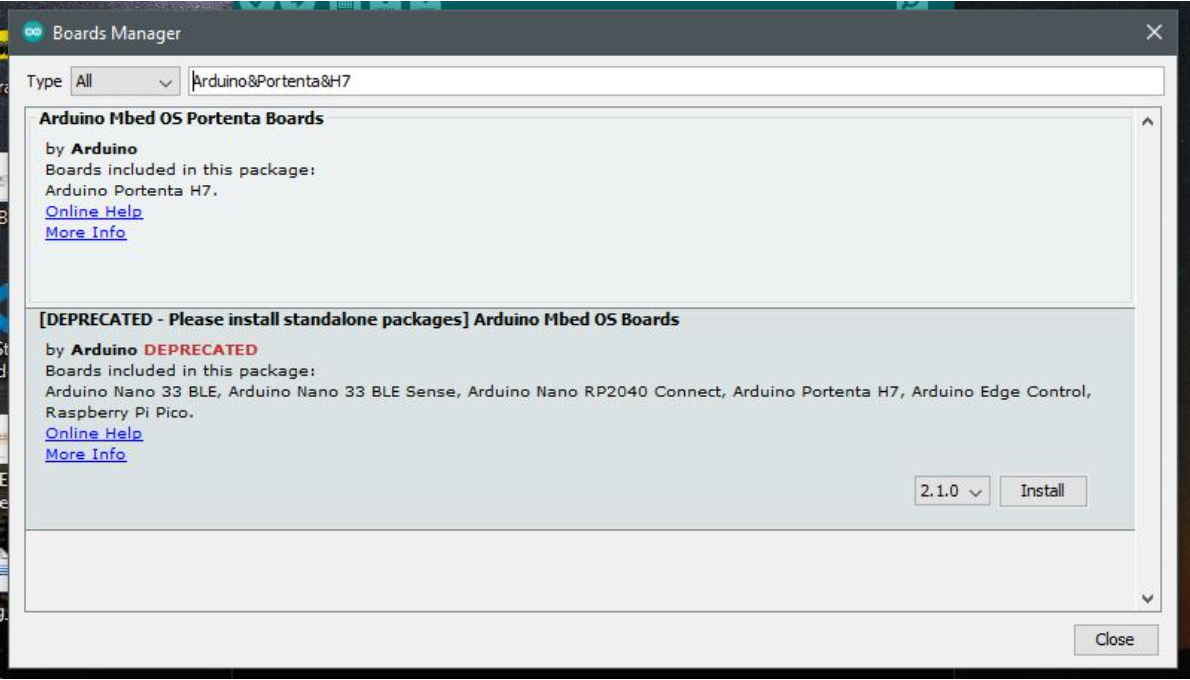
\includegraphics[width=0.7\linewidth]{Images/ArduinoIDE/ArduinoPackage.png}
			\caption{Install packages for Arduino PortentaH7}
			\label{ArduinoPackage}
		\end{center}
	\end{figure}
\end{comment}


\subsection{Example Blink Sketch}

To upload the example sketch, go to \SHELL{File > Examples > Basics > Blink} as shown in Figure ~\ref{UploadSketch}. \\

\begin{figure}
	\begin{center}
		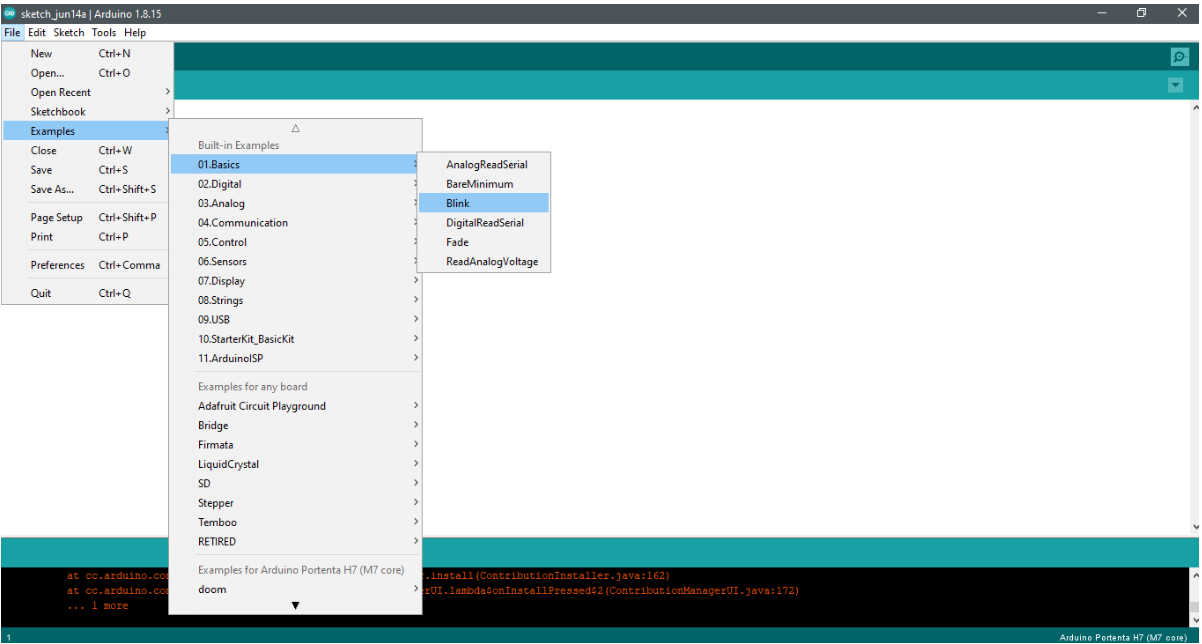
\includegraphics[width=0.7\linewidth]{Images/ArduinoIDE/UploadSketch.png}
		\caption{Upload Basic Sketch}
		\label{UploadSketch}
	\end{center}
\end{figure}

In the program, we initialize \SHELL{LED\_BUILTIN} as the output in the setup function. In the loop function we turn on the LED by using \SHELL{digitalWrite()} function. Click on upload and wait for it to complete. After the upload is done, the green LED on the board starts blinking with a delay of 1000ms. The blink sketch appears on the screen as shown in figure \ref{CompileSketch}.

\begin{code}
	% Include a specific range of lines from the C++ file
	\lstinputlisting[language=C++, firstline=1, lastline=81, label={lst:arduinoBlink}]{../Code/Arduino/ArduinoCLI/BLINK.ino}
\end{code}



\begin{figure}
	\begin{center}
		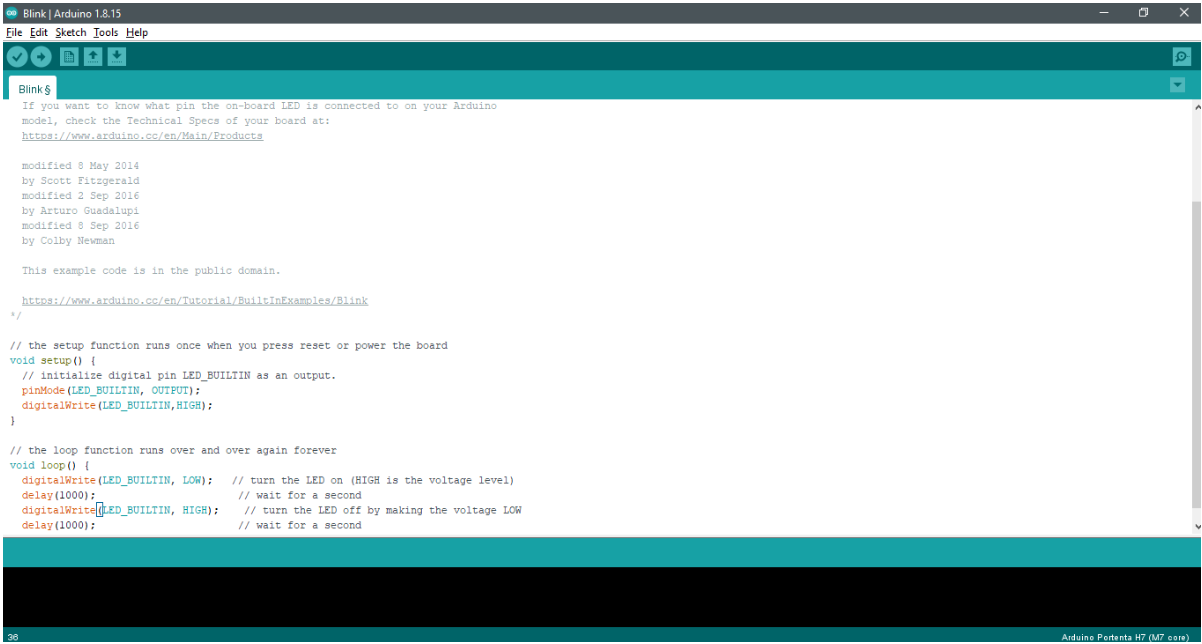
\includegraphics[width=0.7\linewidth]{Images/ArduinoIDE/CompileSketch.png}
		\caption{Compile Blink Sketch}
		\label{CompileSketch}
	\end{center}
\end{figure}

\subsection{Serial Blink Example for Dual Core Processing}

The following figure \ref{SerialBlinkSketch} represents the serial blink sketch. This sketch helps in demonstrating the serial data transmission by showing the LED blinking after a certain time period. \\

Here, \SHELL{Serial.begin(115200)} command sets the data transmission rate to 115200 bits per second. The LEDB is the output which blinks in blue color and we have specified core M7. If we would like to use core M4 then we need to boot it first using bootM4() command. The ouput LED blinks blue in color after a delay of 3 seconds as defined in the sketch. \\

\begin{figure}
	\begin{center}
		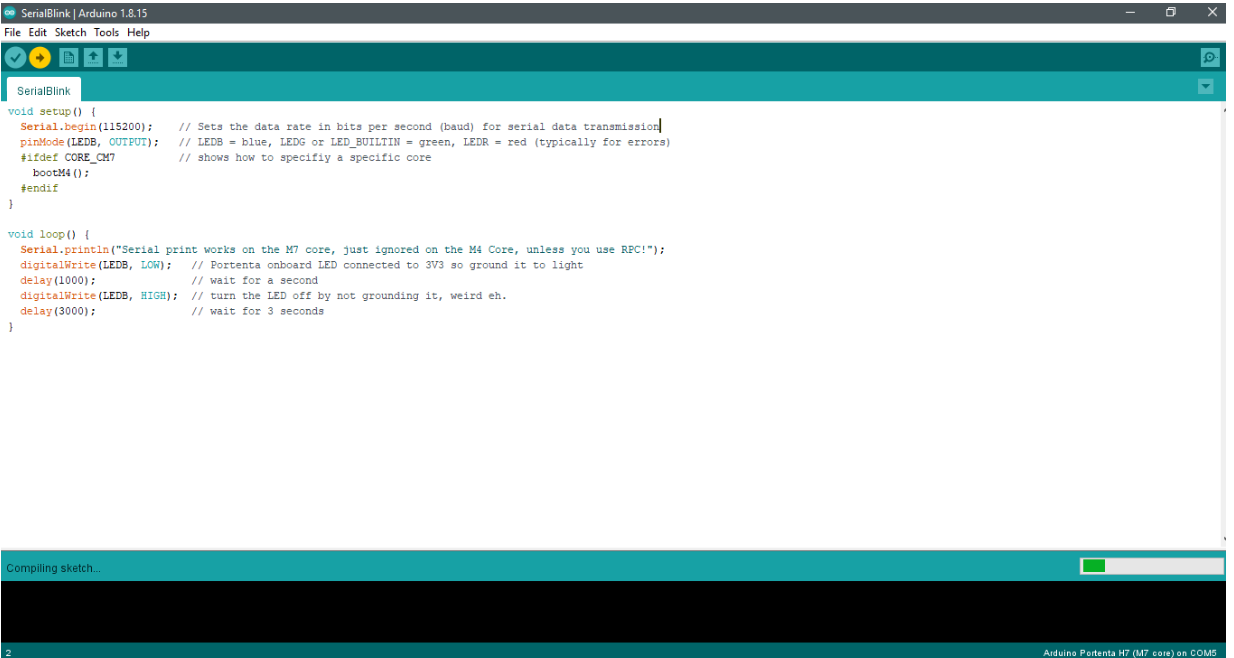
\includegraphics[width=0.7\linewidth]{Images/ArduinoIDE/SerialBlink.png}
		\caption{Serial Blink Sketch}
		\label{SerialBlinkSketch1}
	\end{center}
\end{figure}

In order to use core M4, we need to de-select the core M7 from the board and select core M4. After selecting, we can see at the bottom the selected core for confirmation. Also, We need to write another sketch and now change the LED color to red in the sketch and add a delay of 4 seconds. \\
\begin{figure}
	\begin{center}
		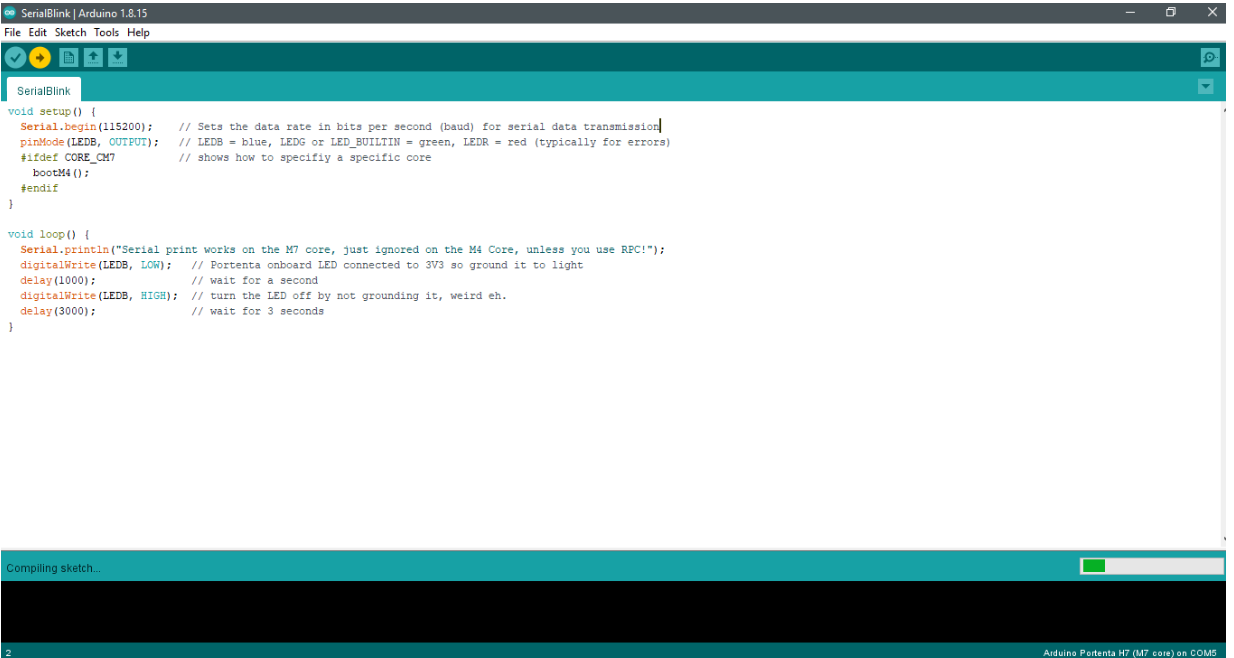
\includegraphics[width=0.7\linewidth]{Images/ArduinoIDE/SerialBlink.png}
		\caption{Serial Blink Sketch}
		\label{SerialBlinkSketch}
	\end{center}
\end{figure}


Notice that in the output both LED blue and green blinks and at a point in time they almost blink together resulting in a Lila color. This shows the dual core processing concept by using an LED. \\

\begin{figure}
	\begin{center}
		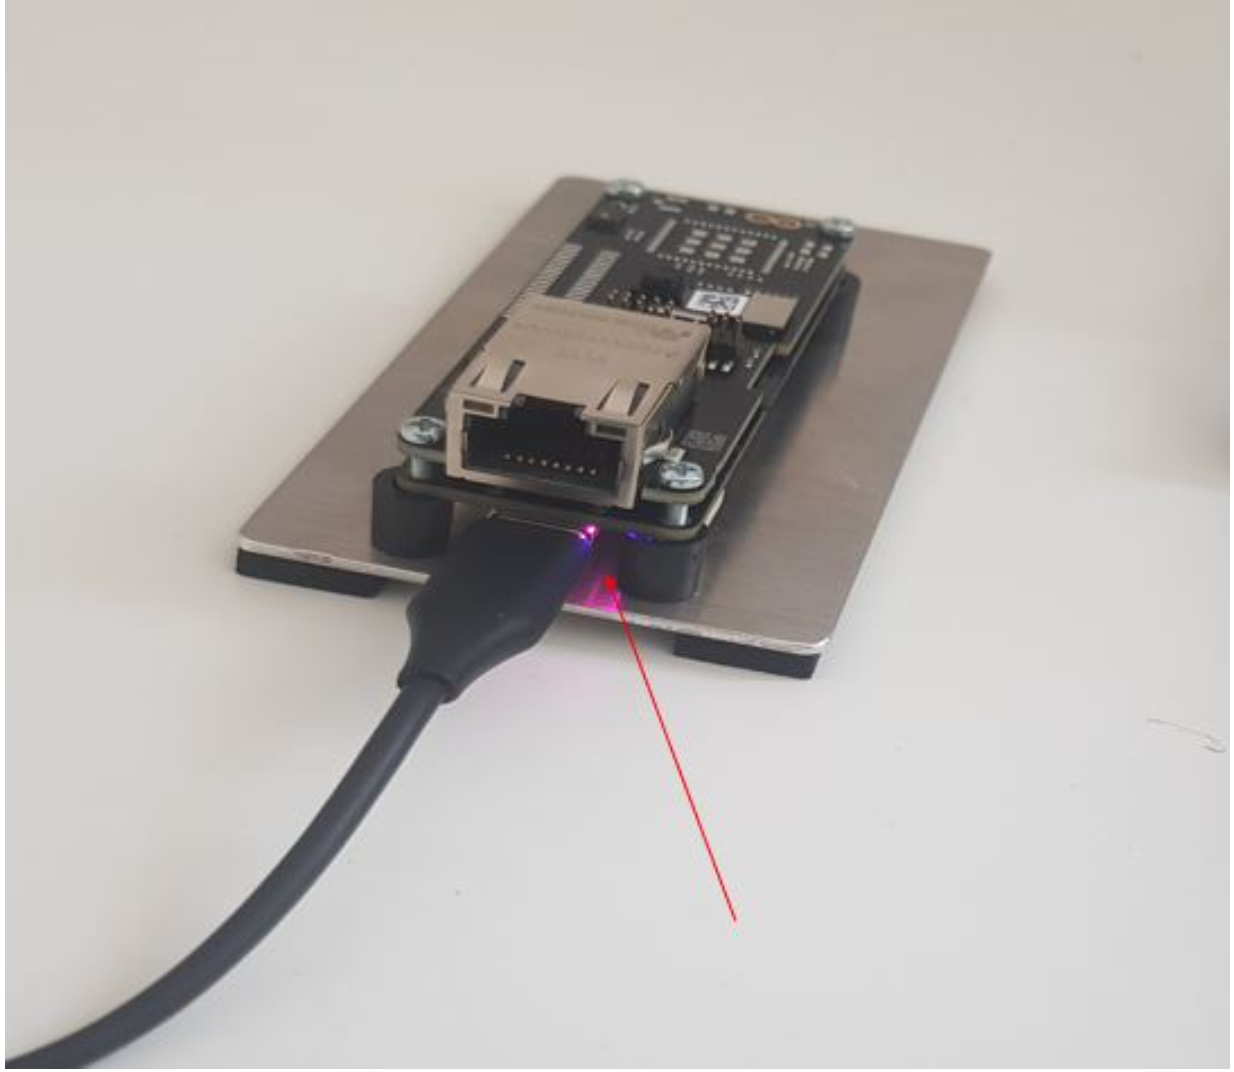
\includegraphics[width=0.7\linewidth]{Images/ArduinoIDE/Output.png}
		\caption{Output LED Color}
		\label{Output}
	\end{center}
\end{figure}

It can be seen from the figure \ref{Output} that the output LED blinks in Lila color due to the overlapping of the green and blue LED blinking at the same time.